\documentclass{report}

% Paquetes y configuraciones adicionales
\usepackage{graphicx}
\usepackage[export]{adjustbox}
\usepackage{caption}
\usepackage{float}
\usepackage{titlesec}
\usepackage{geometry}
\usepackage[hidelinks]{hyperref}
\usepackage{titling}
\usepackage{titlesec}
\usepackage{parskip}
\usepackage{wasysym}
\usepackage{tikzsymbols}
\usepackage[spanish]{babel}

\newcommand{\subtitle}[1]{
  \posttitle{
    \par\end{center}
    \begin{center}\large#1\end{center}
    \vskip0.5em}
}

% Configura los márgenes
\geometry{
    left=2cm,   % Ajusta este valor al margen izquierdo deseado
    right=2cm,  % Ajusta este valor al margen derecho deseado
    top=3cm,
    bottom=3cm,
}

% Configuración de los títulos de las secciones
\titlespacing{\section}{0pt}{\parskip}{\parskip}
\titlespacing{\subsection}{0pt}{\parskip}{\parskip}
\titlespacing{\subsubsection}{0pt}{\parskip}{\parskip}

% Redefinir el formato de los capítulos y añadir un punto después del número
\makeatletter
\renewcommand{\@makechapterhead}[1]{%
  \vspace*{0\p@}% Ajusta este valor para el espaciado deseado antes del título del capítulo
  {\parindent \z@ \raggedright \normalfont
    \ifnum \c@secnumdepth >\m@ne
        \huge\bfseries \thechapter.\ % Añade un punto después del número
    \fi
    \interlinepenalty\@M
    #1\par\nobreak
    \vspace{10pt} % Ajusta este valor para el espacio deseado después del título del capítulo
  }}
\makeatother

\begin{document}

% Portada del informe

\title{Práctica 07. Una configuración sencilla de Firewall con IPtables}
\subtitle{Seguridad de Sistemas Informáticos}
\author{Cheuk Kelly Ng Pante}
\date{\today}

\maketitle

% Índice
\tableofcontents

% Nueva página para el primer capítulo
\cleardoublepage

% Secciones del informe
\chapter{Configurar las interfaces de red del firewall}
Para este punto debemos activar dos interfaces de red, esto lo hicimos en la práctica anterior, ya que una de las interfaces (DOCINT1) no se configuró ya que no teníamos la IP. En mi caso he seleccionado la IP 192.168.10.0/24. Para configurar la interfaz DOCINT1, ens4 en la MV del firewall, vamos a configurar el fichero \emph{/etc/network/interfaces} y metemos lo siguiente:

\begin{verbatim}
auto ens4
iface ens4 inet static
  address 192.168.10.1
  netmask 255.255.255.0
  \end{verbatim}

Una vez añadido la configuración reiniciamos lo servicios de red con el siguiente comando:

\begin{verbatim}
usuario@debian# sudo systemctl restart networking
  \end{verbatim}

Una vez reiniciado ya tenemos configurado la interfaz que se utilizará para trabajar sobre una red privada. Aqui una captura de pantalla de la configuración hecha:

\begin{figure}[H]
  \centering
  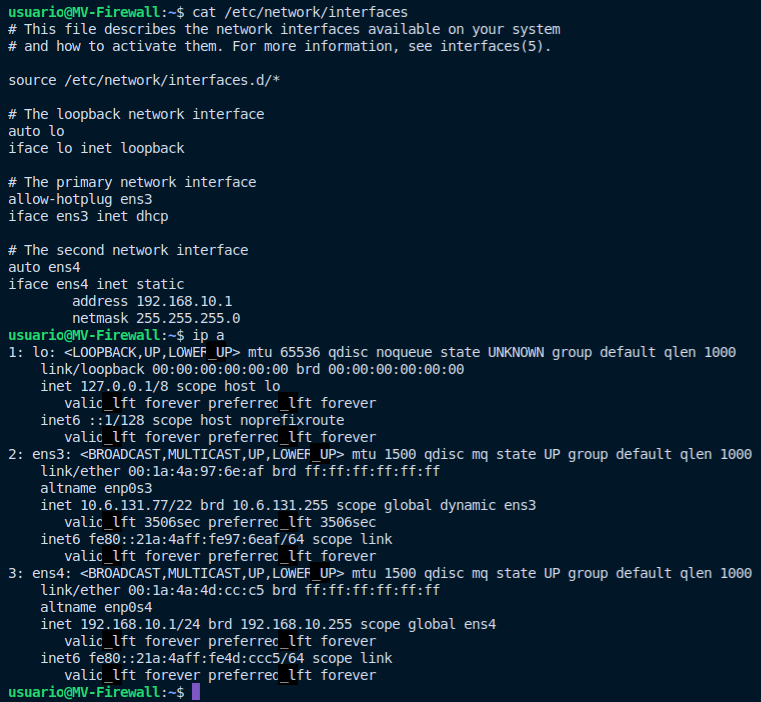
\includegraphics[scale=0.6]{img/configuracion_interfaces_firewall.png}
  \caption{Configuración de las interfaces de red}
  \label{fig:configuracion_interfaces}
\end{figure}

% Nueva página 
\cleardoublepage

\chapter{Asignar máquina virtual “cliente” como cliente}
Para este punto vamos a configurar el fichero \emph{/etc/network/interfaces} de la máquina virtual “cliente” y configuramos otra segunda interfaz y hacemos lo mismo que en el apartado anterior con la única diferencia que en esta interfaz que vamos a configurar añadimos un gateway que va a ser la de la “Red interna”.
El \emph{/etc/network/interfaces} vamos a añadir los siguiente:

\begin{verbatim}
auto ens8
iface ens8 inet statis
  address 192.168.10.2
  netmask 255.255.255.0
  gateway 192.168.10.1
  \end{verbatim}

Una vez añadido la configuración reiniciamos lo servicios de red con el siguiente comando:

\begin{verbatim}
usuario@debian# sudo systemctl restart networking
  \end{verbatim}

\begin{figure}[H]
  \centering
  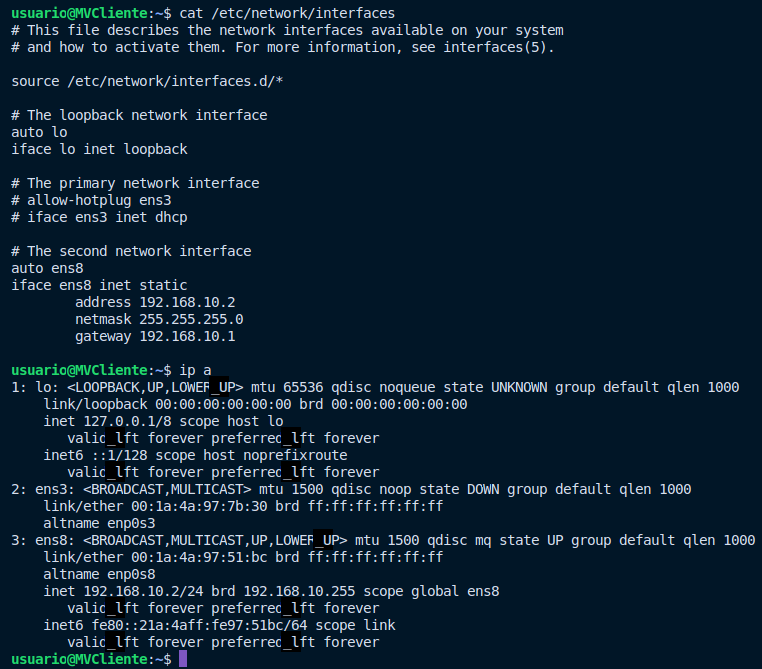
\includegraphics[scale=0.65]{img/configuracion_interfaces_cliente.png}
  \caption{Configuración de las interfaces de red}
  \label{fig:configuracion_interfaces_cliente}
\end{figure}

A continuación, instalamos un navegador en modo texto, en este caso instalamos \emph{links} y lo hacemos de la siguiente manera:

\begin{verbatim}
usuario@debian# sudo apt install links
  \end{verbatim}

\begin{figure}[H]
  \centering
  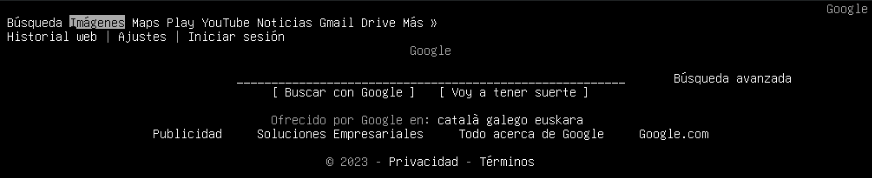
\includegraphics[scale=0.65]{img/links_google.png}
  \caption{Captura de pantalla del navegador \emph{links}}
  \label{fig:links}
\end{figure}

\chapter{Configurar el Firewall}
\begin{itemize}
  \item Tenga política por defecto ACCEPT para la cadena OUTPUT y DROP para INPUT y FORWARD:

  \begin{verbatim}
    iptables -P INPUT DROP
    iptables -P FORWARD DROP
    iptables -P OUTPUT ACCEPT
  \end{verbatim}
  
  \item Permita conectividad total desde la interfaz de loopback (lo) para hacer pruebas desde la consola del firewall:
  
  \begin{verbatim}
    iptables -A INPUT -i lo -j ACCEPT
  \end{verbatim}
  
  \item Acepte conexiones desde la red interna a los puertos 80 (web) y 22 (servicio SSH en el FW)
  
  \begin{verbatim}
    iptables -A INPUT -p tcp --dport ssh -j ACCEPT
    iptables -A INPUT -p tcp --sport 80 -j ACCEPT
  \end{verbatim}
  
  \item Crear una cadena "custom" denominada "SERVICES" para la gestión de los servicios anteriores:
  
  \begin{verbatim}
    # Crear la cadena "SERVICES"
    iptables -N SERVICES
  
    # Añadir reglas a la cadena "SERVICES"
    iptables -A FORWARD -i ens4 -s 192.168.10.0/24 -j SERVICES
  
    # Crear una cadena "SERVICES" y agregar reglas a ella
    # Permitir trafico a los puertos 80 y 22
    iptables -A SERVICES -p tcp --dport 22 -j ACCEPT
    iptables -A SERVICES -p tcp --dport 80 -j ACCEPT
    iptables -A SERVICES -p tcp --dport 443 -j ACCEPT
  \end{verbatim}
  
  \item Permita el tráfico a una impresora a todo el rango IP de la clase C especificada en la red interna:
  
  \begin{verbatim}
    iptables -A FORWARD -i ens4 -o ens4 -s 192.168.10.2 -d
    192.168.10.0/24 -j ACCEPT
    iptables -A FORWARD -i ens4 -o ens4 -s 192.168.10.0/24 -d
    192.168.10.2 -j ACCEPT
  \end{verbatim}
\end{itemize}

\begin{figure}[H]
  \centering
  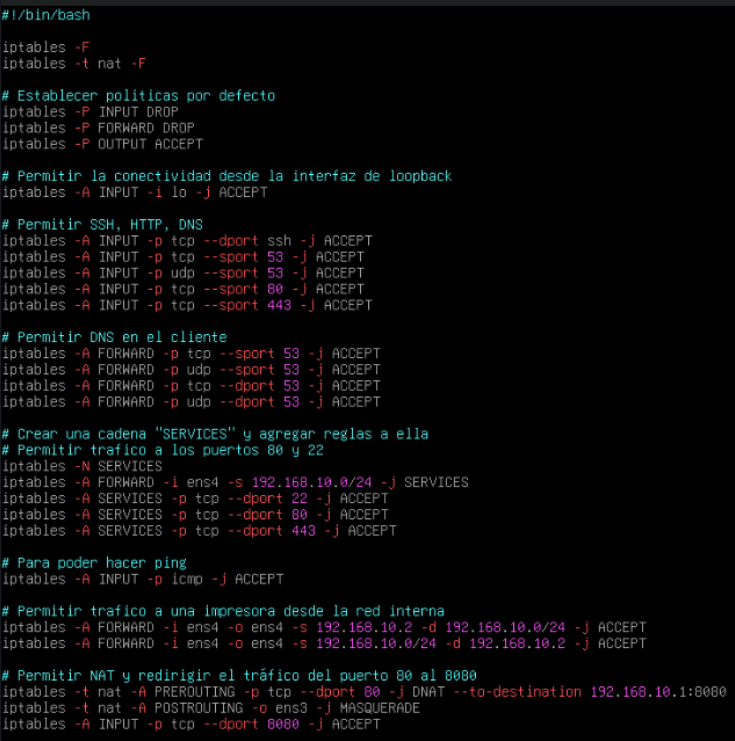
\includegraphics[scale=0.65]{img/firewall.png}
  \caption{Captura de pantalla del script de \emph{firewall}}
  \label{fig:script firewall}
\end{figure}

\chapter{Configuración de un proxy}
Para implementar un proxy transparente para que los clientes de la red interna
puedan navegar por internet vamos a implementar otro script en bash que va a
tener el siguiente contenido:

\begin{verbatim}
!/bin/bash

iptables -t nat -A PREROUTING -p tcp --dport 80 -j DNAT --to-destination 192.168.10.1:8080
iptables -A INPUT -p tcp --dport 8080 -j ACCEPT
iptables -t nat -A POSTROUTING -o ens3 -j MASQUERADE
  \end{verbatim}

Para poder utilizar un proxy transparente para dar servicio de navegación a los
clientes de la red interna, vamos a instalar \emph{Squid Cache}:

\begin{figure}[H]
  \centering
  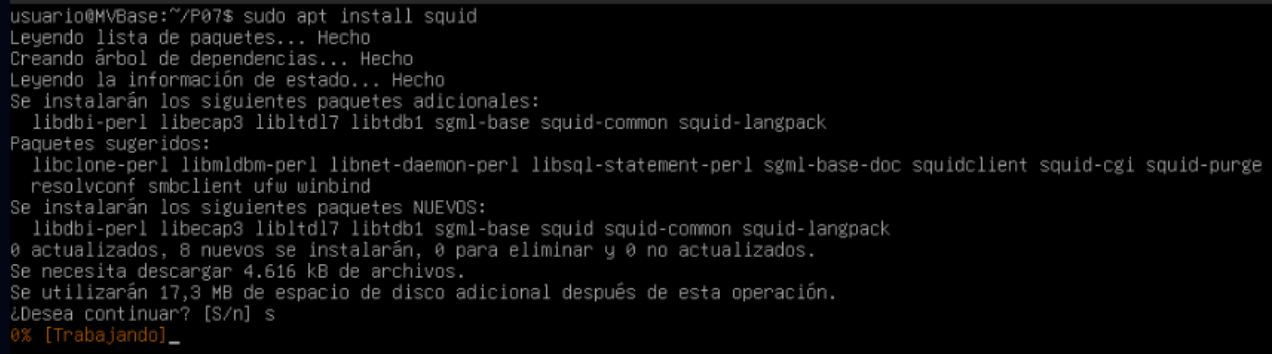
\includegraphics[scale=0.5]{img/squid.png}
  \caption{Instalación del \emph{squid}}
  \label{fig:squid}
\end{figure}

Una vez instalado el \emph{squid} vamos a configurar el fichero /etc/squid/squid.conf y añadimos lo siguiente:

\begin{verbatim}
acl localnet src 192.168.10.0/24
http_port 192.168.10.1:8080 intercept
  \end{verbatim}

y buscamos la línea \emph{http\_access deny CONNECT !SSL\_Ports} y la comentamos, quedandose el fichero de configuracion como se muestra en la figura \ref{fig:squid config}

\begin{figure}[H]
  \centering
  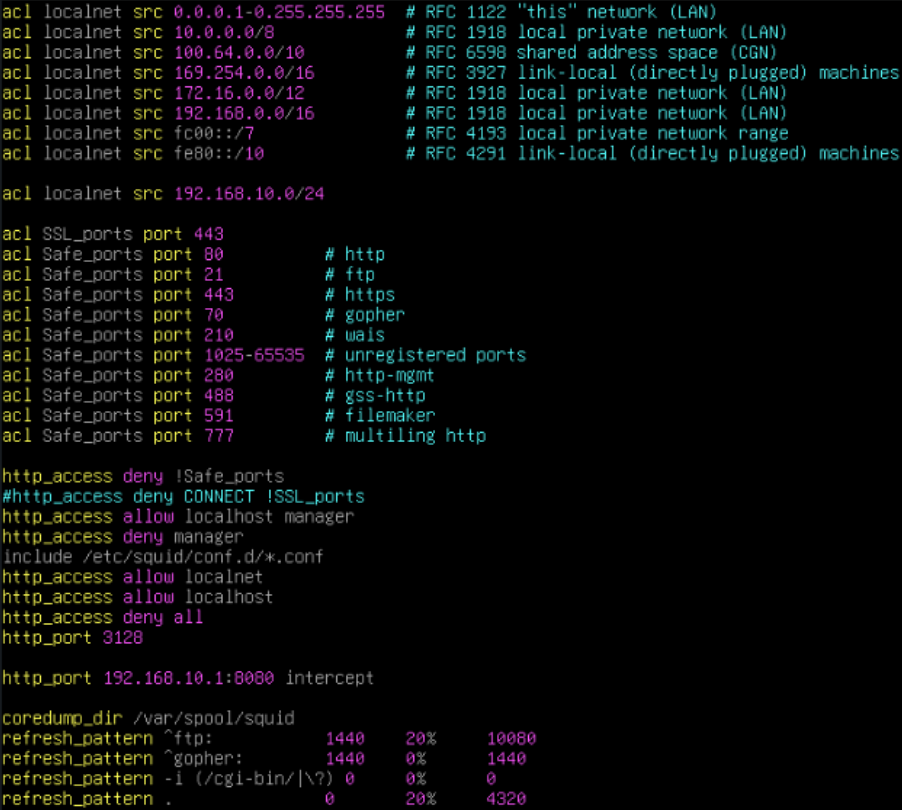
\includegraphics[scale=0.65]{img/config_squid.png}
  \caption{Configuracion del \emph{squid}}
  \label{fig:squid config}
\end{figure}

Ahora, reiniciamos el servicio de \emph{squid}:
\begin{verbatim}
usuario@debian# sudo systemctl restart squid.service
  \end{verbatim}

Una vez que se haya reiniciado probamos en la máquina cliente si hay conexión a internet:

\begin{figure}[H]
  \centering
  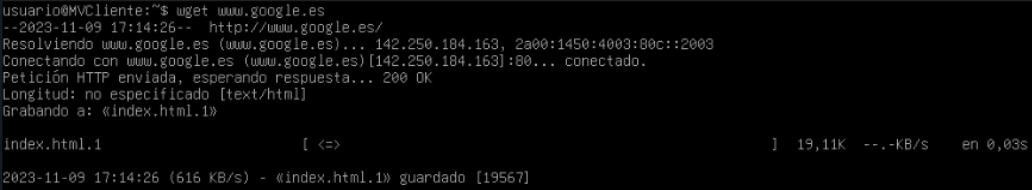
\includegraphics[scale=0.37]{img/wget_google.png}
  \caption{wget a \emph{Google}}
  \label{fig:wget google}
\end{figure}

\cleardoublepage

Otra prueba que podemos hacer es un \emph{curl} a \emph{ull.es}:

\begin{figure}[H]
  \centering
  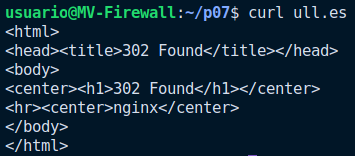
\includegraphics[scale=0.8]{img/curl_ull.png}
  \caption{curl a \emph{ULL}}
  \label{fig:curl ULL}
\end{figure}

Otra prueba que podemos hacer es usar el navegador de texto \emph{links} para ver si podemos navegar por internet:
\begin{figure}[H]
  \centering
  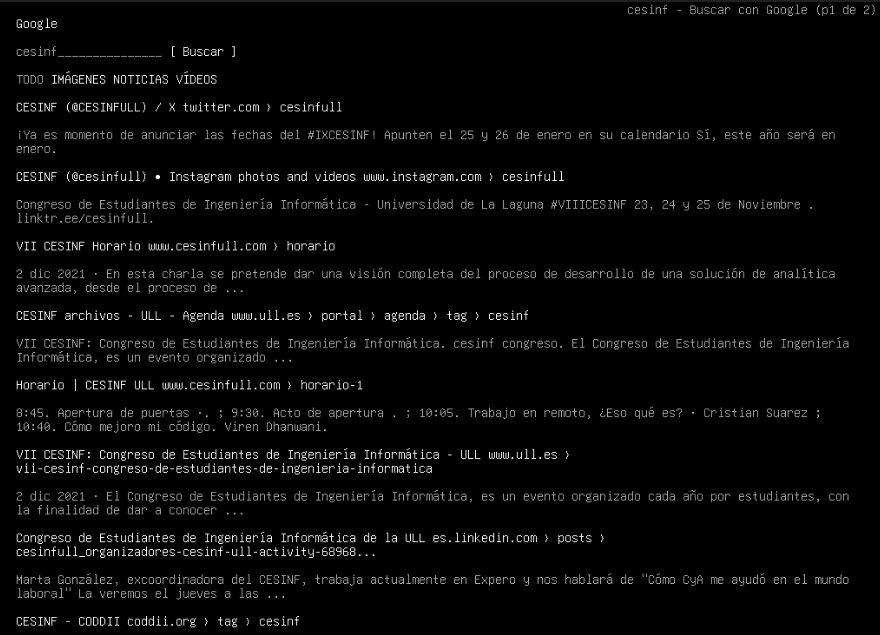
\includegraphics[scale=0.65]{img/links_cesinf.png}
  \caption{Navegación por el navegador de texto \emph{Links}}
  \label{fig:links cesinf}
\end{figure}

\end{document}